\chapter{Packet Formats}~\label{sec:packet-format}
In this section, we describe the SCION header format. The SCION header consists of two parts: the common header and the protocol header. 
The protocol header is defined differently by the contents of a packet. Currently, we have two protocol headers: one for PCBs, and the other one for all other data packets.


\section{Common Header}~\label{subsec:common-header}
All SCION packets have the common header. The common header contains the most basic packet information that is necessary for all SCION packets. The Figure~\ref{fig:hdr-common} shows the common header format.

\begin{figure}[ht]
\centering
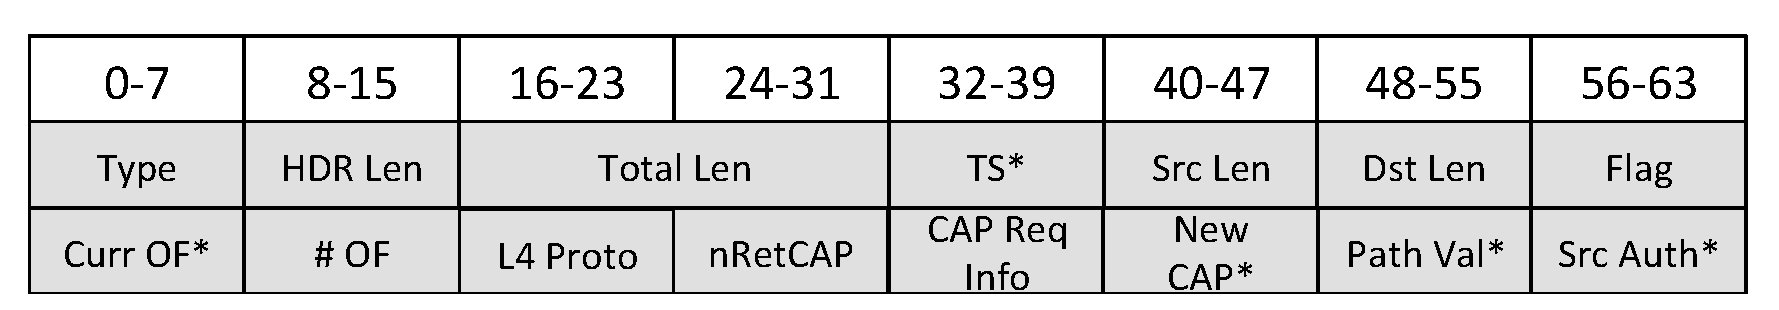
\includegraphics[width=.9\columnwidth]{./fig/nhdr_common.eps}
\caption{Common Header.}\label{fig:hdr-common}
\end{figure}

\begin{itemize}
\item{Type: } BEACON, DATA, CERT\_REQ, CERT\_REP, PATH\_REG, PATH\_REQ, PATH\_REP
\item{HDR Len: } Common header length
\item{Total Len: } Total packet length (including header)
\item{TS*: } Pointer (or offset in Bytes from the beginning of payload) to the current timestamp. Note: up-path and down-path have different timestamps marked by different TDC ADs. The first router on the down-path updates this pointer with the offset to the special opaque field that contains down-path timestamp.
\item{Src Len: } The length of source address, e.g., 4B for IPv4 and 16B for IPv6. Any (new) address can be supported. This field can be zero for special control-plane messages (e.g., BEACON message does not require the source address). 
\item{Dst Len: } The length of destination address. This field can be updated by border routers if they put an internal server's address. For example, if a border router receives a BEACON message, the router sets the Beacon Server's address to the destination address field and its size to the Dst Len field. 
\item{Flag: } Path status information. Each bit (from the MSB) has the following meanings -- (0) up/down path, (1) overuse, (2) congestion.\footnote{overuse and congestion bits are used in STRIDE (i.e., SCION DDoS extension).} 
\item{Current OF*: } The pointer to the current opaque field. An ingress router (of an AD) processes a data packet with the opaque field specified in this pointer.
\item{\# OF: } number of opaque fields in the current marking. This would be used for an offset to the capability field.
\item{L4 Proto: }  Upper-layer transport protocol, e.g., TCP, UDP
\item{nRetCap: } The size of the return capability (which consists of a series of router capabilities). 
\item{Cap Req Info: } Capability request information
\item{New CAP*: } Offset to the new capabilities. If the packet type is capability request (CAP\_REQ) or renewal (CAP\_RENEW), routers on the forwarding path write new capabilities in this field.
\item{Path Val*: } Pointer to the {\em path validation} information (variable size)
\item{Source Auth*: } Pointer to the {\em source authorization} information (variable size)
\end{itemize}


\section{Beacon Header}
An \AD's beacon server, when it receives a PCB from its provider \AD, adds its own marking and signature to the PCB; and forwards the PCB to its customer \AD. Hence, a PCB eventually constructs a path from \ISDC to an \STUB \AD. Figure~\ref{fig:hdr-beacon} shows the beacon header format.

\begin{figure}[ht]
\centering
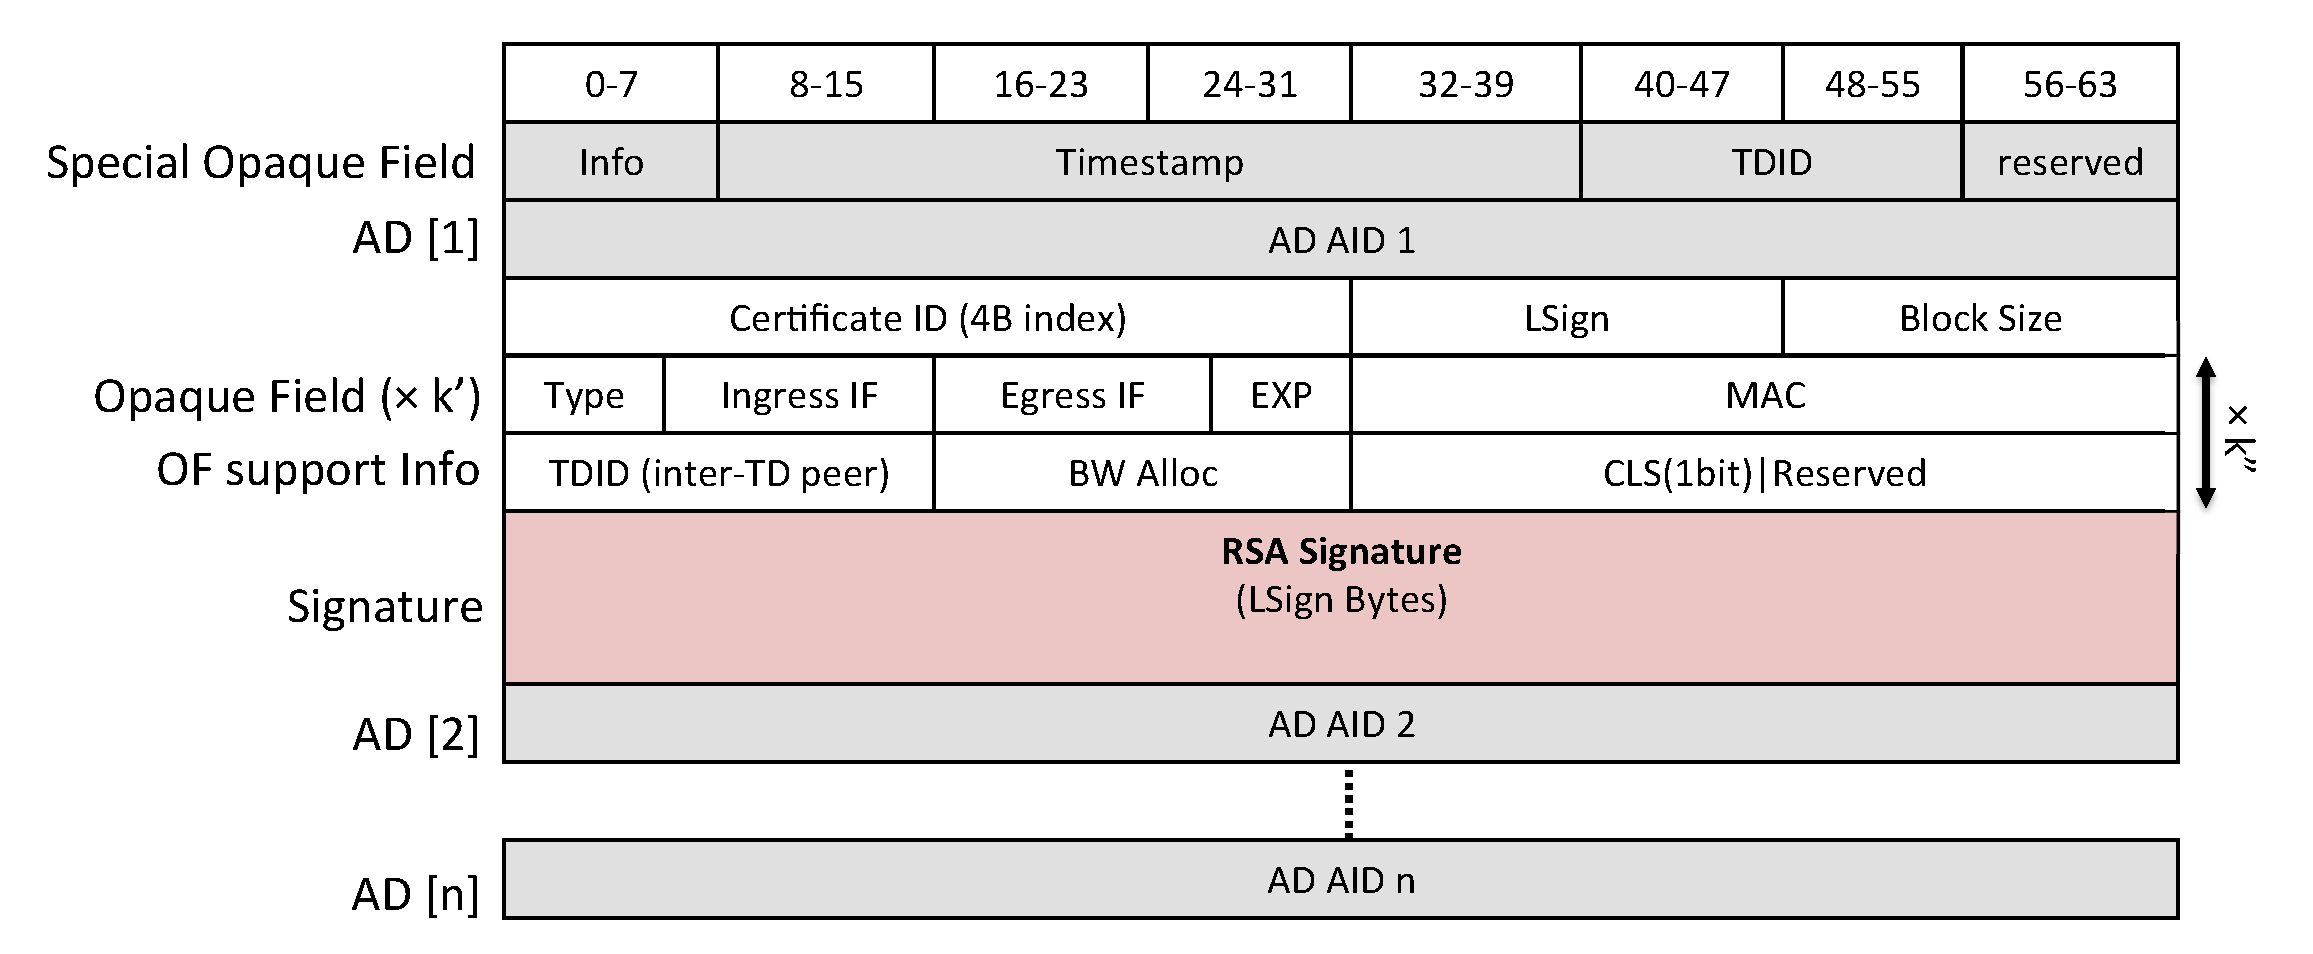
\includegraphics[width=.9\columnwidth]{./fig/nhdr_pcb.eps}
\caption{Beacon Header.}\label{fig:hdr-beacon}
\end{figure}

\begin{itemize}
\item{Info: }This field is used for data packets. To make the opaque field format consistent (i.e., 8B aligned) over all opaque fields.
\item{Timestamp: }PCB's timestamp marked by its initiator (i.e., \ISDC \BS).
\item{AD AID: } authenticated ID of an \AD (this can be the hash of an AD's public key).
\item{Certificate ID: } ID of the certificate (i.e., the signed public key) used for RSA signature generation. Change of this value signals the change of the current AD's certificate and would have BSs retrieve the new certificate from the \CS.
\item{LSign: } signature length; e.g., 1024 bits, 2048 bits
\item{Block Size: } the total size of block marked by an \AD (in bytes), which determines the offset from which a new AD marking starts
\item{Type (4 bits): } This field indicates whether the current opaque field continues in the next opaque field or not. Zero in the MSB indicates the current opaque field is the end of the opaque field. If an AD needs more than 8B for its marking, it set the MSB and add more information to the next 8B, thereby the AD can use several 8B-aligned opaque field blocks. 
\item{Ingress IF (13 bits): } ingress interface id (internal use)
\item{Egress IF (13 bits): } egress interface id (internal use), or egress interface of peer (for a peering link, the egress interface to the customer AD is same as that of the first opaque field because a PCB is send to a single egress interface)
\item{EXP (2 bits): } lifetime of the path; current assignment: 00 - 6HR, 01 - 12HR, 10 - 18HR, 11 - 24HR
\item{MAC: } Massage Authentication Code, MAC(i) = $AES-CBC-MAC_{K_i}$(Ingress IF$||$Egress IF$||$OF(i-1)$||$ AD$_{next}$) \newline
	$K_i$ – MAC generation key of AD[i], AD$_{next}$ is the AD[i]'s customer to which the PCB is forwarded. MAC chaining would prevent (malicious) splicing of opaque fields.
\item{ISD ID: } Trusted Domain ID, which is used only for Inter-ISD peering link
\item{Signature: } RSA signature signed by AD[i]
\end{itemize}

An \AD can add all its peering links to a PCB. The \BS, when it constructs an opaque field for a peering link, fills the Egress IF field with that of the peer so that the \STUB \AD can find an interface-level shortcut. However, the MAC of a peering link should not be computed with the Egress IF field but be computed with the Egress IF to which a PCB propagates. Since the opaque field of a non-peering link (i.e., the opaque field for the path from \ISDC) has the actual egress interface ID, the \BS uses this egress IF in generating the MAC of a peering link. An \STUB \AD, when it constructs a path using a peering link, the \AD writes the egress IF of the opaque field of the peering link with the one used for the MAC generation. And, the \BS does not incorporate the previous \AD's opaque field (i.e., OF(i-1)) in generating the MAC of a peering link since OF(i-1) would not be present at the SCION header when a \STUB \AD constructs a path (i.e., a series of opaque field) using a peering link. An \AD generates its signature by (1) computing a MAC using its markings (including those for the peering links) and the next-hop AD's AID as inputs and (2) then encrypting the message digest with its RSA private key.

\section{Data Header}\label{subsec:data-header}
A data packet, in addition to the common header, carries a series of Opaque Fields that represent an end-to-end path collectively.

\begin{figure}[ht]
\centering
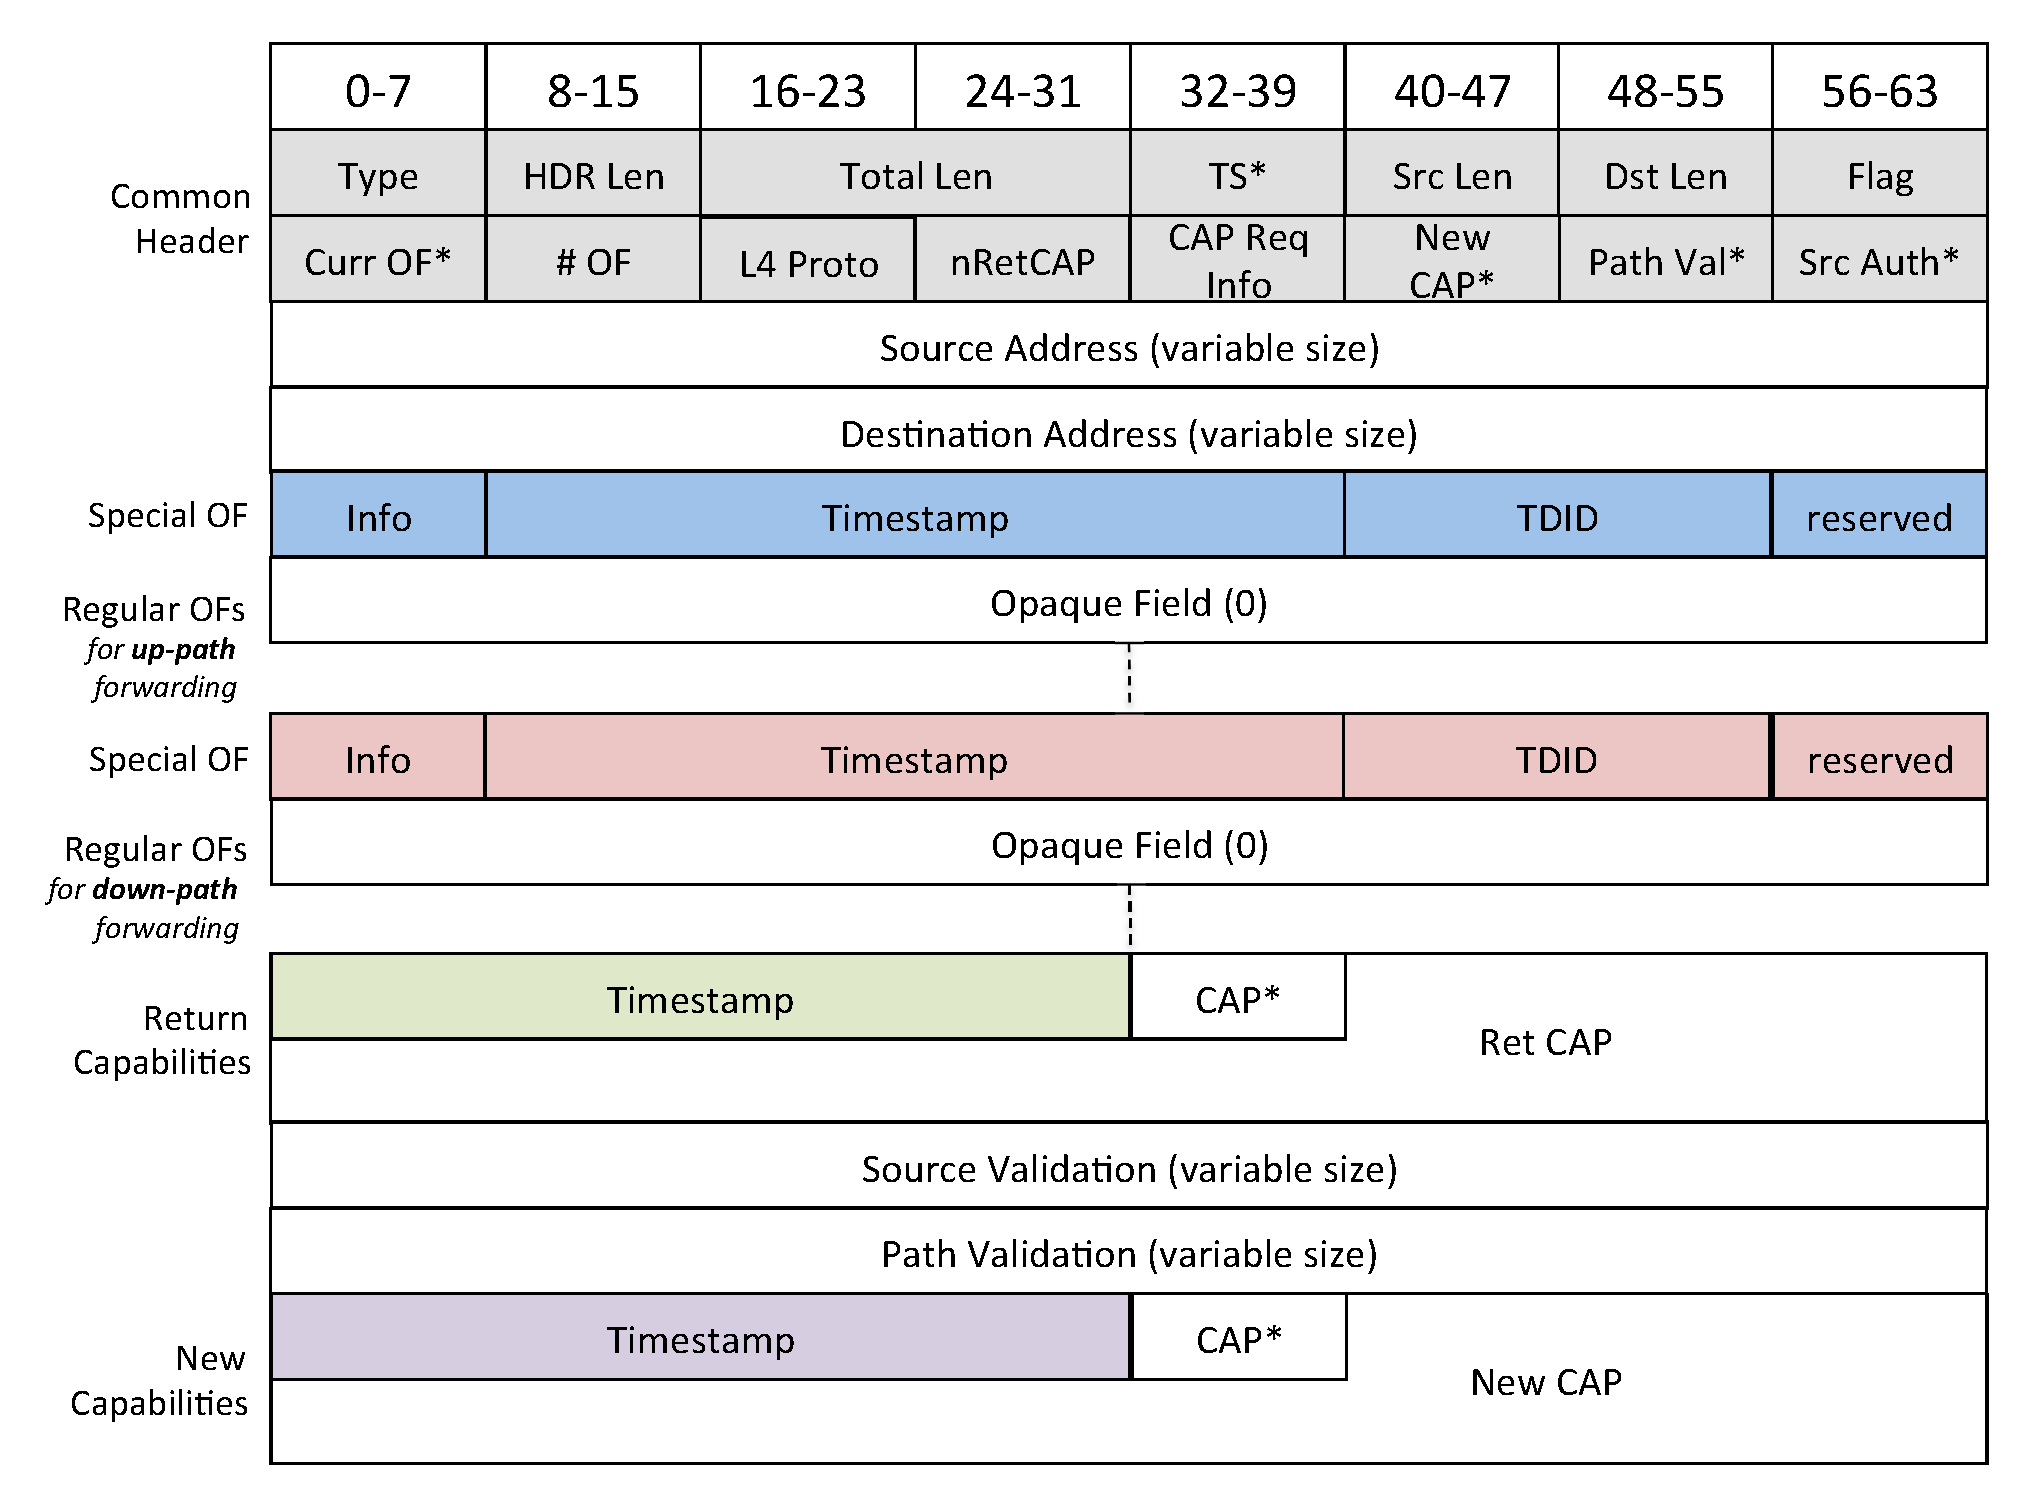
\includegraphics[width=.9\columnwidth]{./fig/nhdr_data.eps}
\caption{Data Header.}\label{fig:hdr-data}
\end{figure}

\begin{itemize}
\item{Special Opaque Field: }This opaque field contains the timestamp that \ISDC \AD marked into the PCB and the isolation domain ID the \AD belongs to. Since this timestamp is valid for a half-path (i.e., from \ISDC to an \STUB \AD), at least two timesstamps (one for up-path and one for down-path) are present in a packet. If a packet traverses multiple \ISDs, it should contain as many timestamps as the number of \ISDs. Info field contains the information regarding a series of opaque fields that use the same timestamp and informs ADs on the path of how to handle opaque fields. Note: Special opaque field processing is required if an \AD is at the crossover point (i.e., at the point where up-path to down-path transition occurs). Info field has the following meanings.
	\begin{itemize}
	\item{0xxxxxxx}: Normal opaque field. A router processes a single opaque field.
	\item{1xxxxxxx}: Special opaque field. The next byte starts with a 4B timestamp. The ingress router has to update the OF* in the common header with the current (special) opaque field.
	\item{10xxxxxx}: Normal ISD core path (i.e., source \AD $\rightarrow$ TDC $\rightarrow$ destination \AD).
	\item{11xxxxxx}: Shortcut path.
	\item{110xxxxx}: Normal shortcut through a common AD of up- and down-path.
	\item{111xxxxx}: Normal shortcut (in-path, viz., example in Figure~\ref{})
	\item{1111xxxx}: Shortcut through a peering link between ASs.
	\item{11110xxx}: Intra-ISD peering link
	\item{11111xxx}: Inter-ISD peering link
	\end{itemize}
Reserved field can be used to specify the size of each opaque field block (i.e., up-path block, down-path block, TDC path block). Using this block size, ADs can quickly identify {\em ISD path} if necessary.
\item{Regular Opaque Field: }Regular opaque fields are used for each router in forwarding packets. A router verifies a packet's MAC with the embedded ingress and egress interface information and if the MAC is correct, the router forwards the packet to the egress interface.
	\begin{itemize}
	\item{Type (4 bits): } Opaque field type. 
		\begin{itemize}
		\item{00xx}: End (indicate the current opaque field ends here). Note: an AD can write multiple blocks of opaque field.
		\item{01xx}: Continue (indicates the current opaque fields continues in the next 8B).
		\item{001x}: Crossover point (inform a router to handle more opaque field based on the crossover type). Crossover point must be specified in all packets.
		\end{itemize}
	\item{Ingress IF (13 bits): } ingress interface id (internal use)
	\item{Egress IF (13 bits): } egress interface id (internal use)
	\item{EXP (2 bits): } Expiration time of the Opaque Field (00: 6 hours, 01: 12 hours, 11: 18 hours, 11: 24 hours)
	\item{MAC (32 bits): } Massage Authentication Code, MAC(i) = $AES-CBC-MAC_{K_i}$(Ingress IF$||$Egress IF$||$OF(i-1)$||$AIDi+1)\newline
		$K_i$ – MAC generation key of AD[i]
	\end{itemize}
Type field is written by the sender of a packet, hence is not used for MAC computation.
\end{itemize}

\section{Examples}
In this section, we illustrate how an \AD establishes an end-to-end path under different topologies. Examples use a simple topology where a half-path from the \ISDC to an \STUB \AD includes four \ADs. We define {\em the number of \ADs on a path} as the path length (i.e., the half-path length is 4 in our examples). A \ISDC \AD is denoted by TDC and all other \ADs are denoted by OP followed by a number, where the OP and number indicate Opaque Field and AD ID respectively. For example, OP01 is the opaque field generated by \AD0 01 for an ingress-egress pair. If \AD 01 generated another opaque field for a different pair of interfaces, the corresponding opaque field is denoted by OP01'.

%1) Up-path and down-path do not have any common \AD but \ISDC.
\subsection{Up-path and down-path do not have any common \AD but \ISDC}

\begin{figure}[h]
\centering
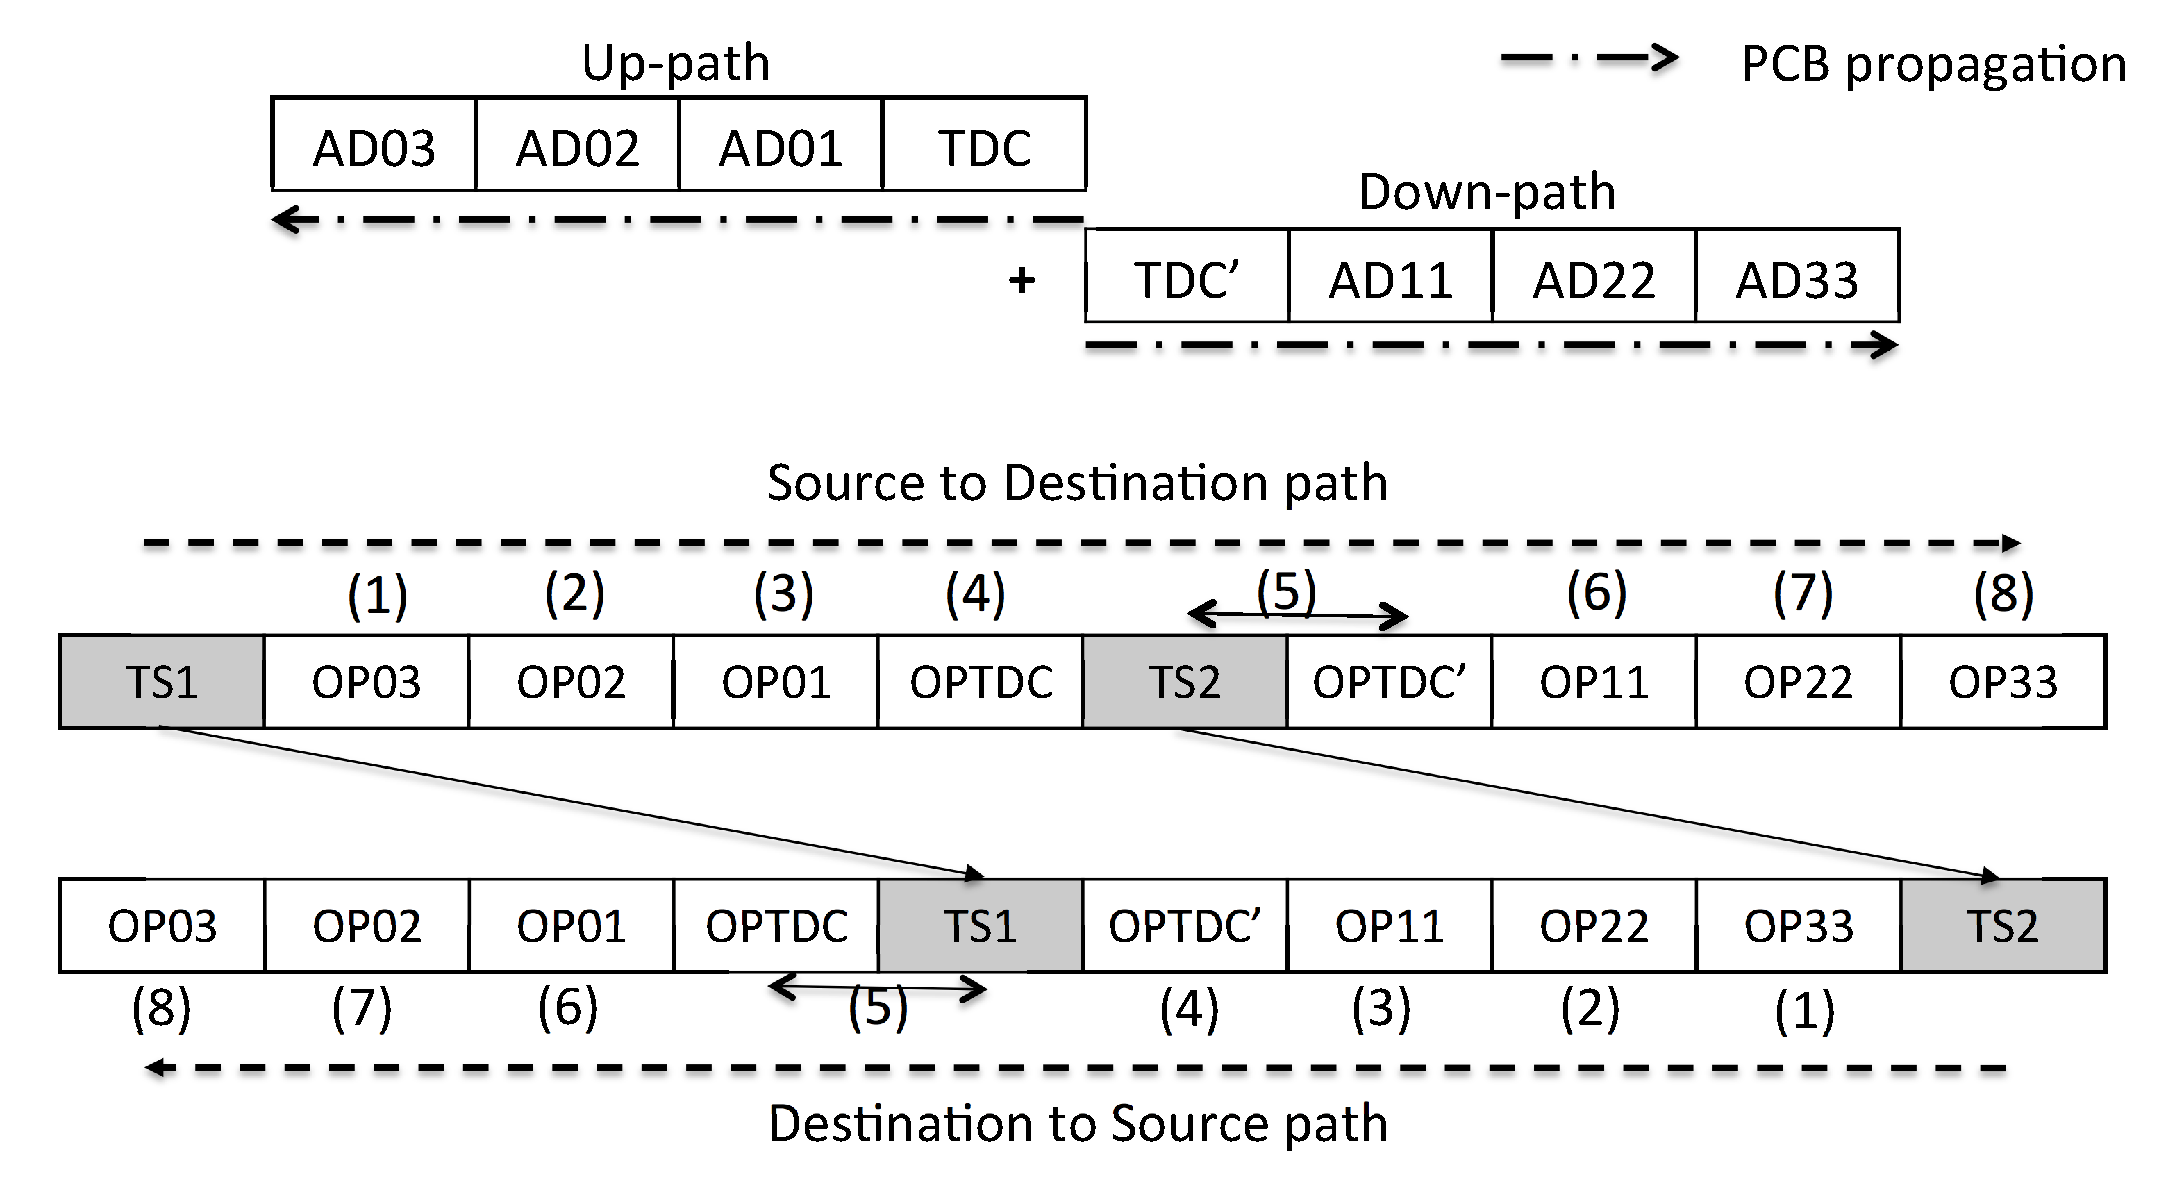
\includegraphics[width=.9\columnwidth]{./fig/nex_fwd1.eps}
\caption{Typical path through \ISDC.}\label{fig:ex-fwd-typical}
\end{figure}

\noindent A sender embeds a series of up-path opaque fields (from its own \AD to \ISDC \AD) and a series of down-path opaque fields (from \ISDC \AD to the destination \AD) into the packet header, thereby constructing a full source to destination path. The up-path opaque field starts with the up-path timestamp (i.e., the special timestamp) so that routers on the path can verify their opaque fields using the timestamp. Similarly, down-path opaque fields start with the down-path timestamp. After embedding the opaque fields, the sender sets the current opaque field pointer (i.e., Curr OF* in Figure~\ref{fig:hdr-common}) to the first opaque field, namely the up-path timestamp. When an \AD sees the special timestamp, the \AD updates the timestamp pointer (i.e., TS*) in the common header and then locates its opaque field by increasing the pointer by 8B. Each \AD on the path locates its own opaque field(s)\footnote{An AD can have multiple opaque fields.} in the common header using the {\em current opaque} field pointer, verifies the opaque field(s): ingress interface ID (i.e., whether the packet arrived at the correct interface) and MAC. If the packet passes the verification, the ingress router increases the opaque field pointer by the amount of its marking, and forwards the packet directly to the egress interface specified in the opaque field. Note that an \AD may have multiple opaque fields that needs to be processed by different routers, hence all routers have to increase opaque field pointer (to the next opaque field) after processing their own part. While all \ADs process opaque field in the same manner, the ingress router of \ISDC \AD (more generally, the ingress router at the end of up-path, which we call the {\em crossover} point) needs to process the opaque field differently. The router has a single egress interface (which an up-path would use as an ingress interface to \ISDC \AD), hence the router has to look at the next opaque field that belong to the first router of the down-path (which would process OPTDC' in the figure), and forwards the packet to the corresponding router. If TDC and TDC' are different \ISDC \ADs, the ingress router of a \ISDC \AD should be able to forward the packet to the next \ISDC \AD. We assume that \ISDC \ADs are well connected and know how to forward packets with each other. When the first router on the down-path receives this packet, the router would see the special opaque field much like the first router on the up-path. Hence, the router would process the packet exactly same way describe before (i.e., update TS* and process its opaque field). The rest of down-path forwarding is exactly same as that of the up-path. 



%2) Up-path and down-path have a common \AD.
\subsection{Up-path and down-path have a common \AD}

\begin{figure}[h]
\centering
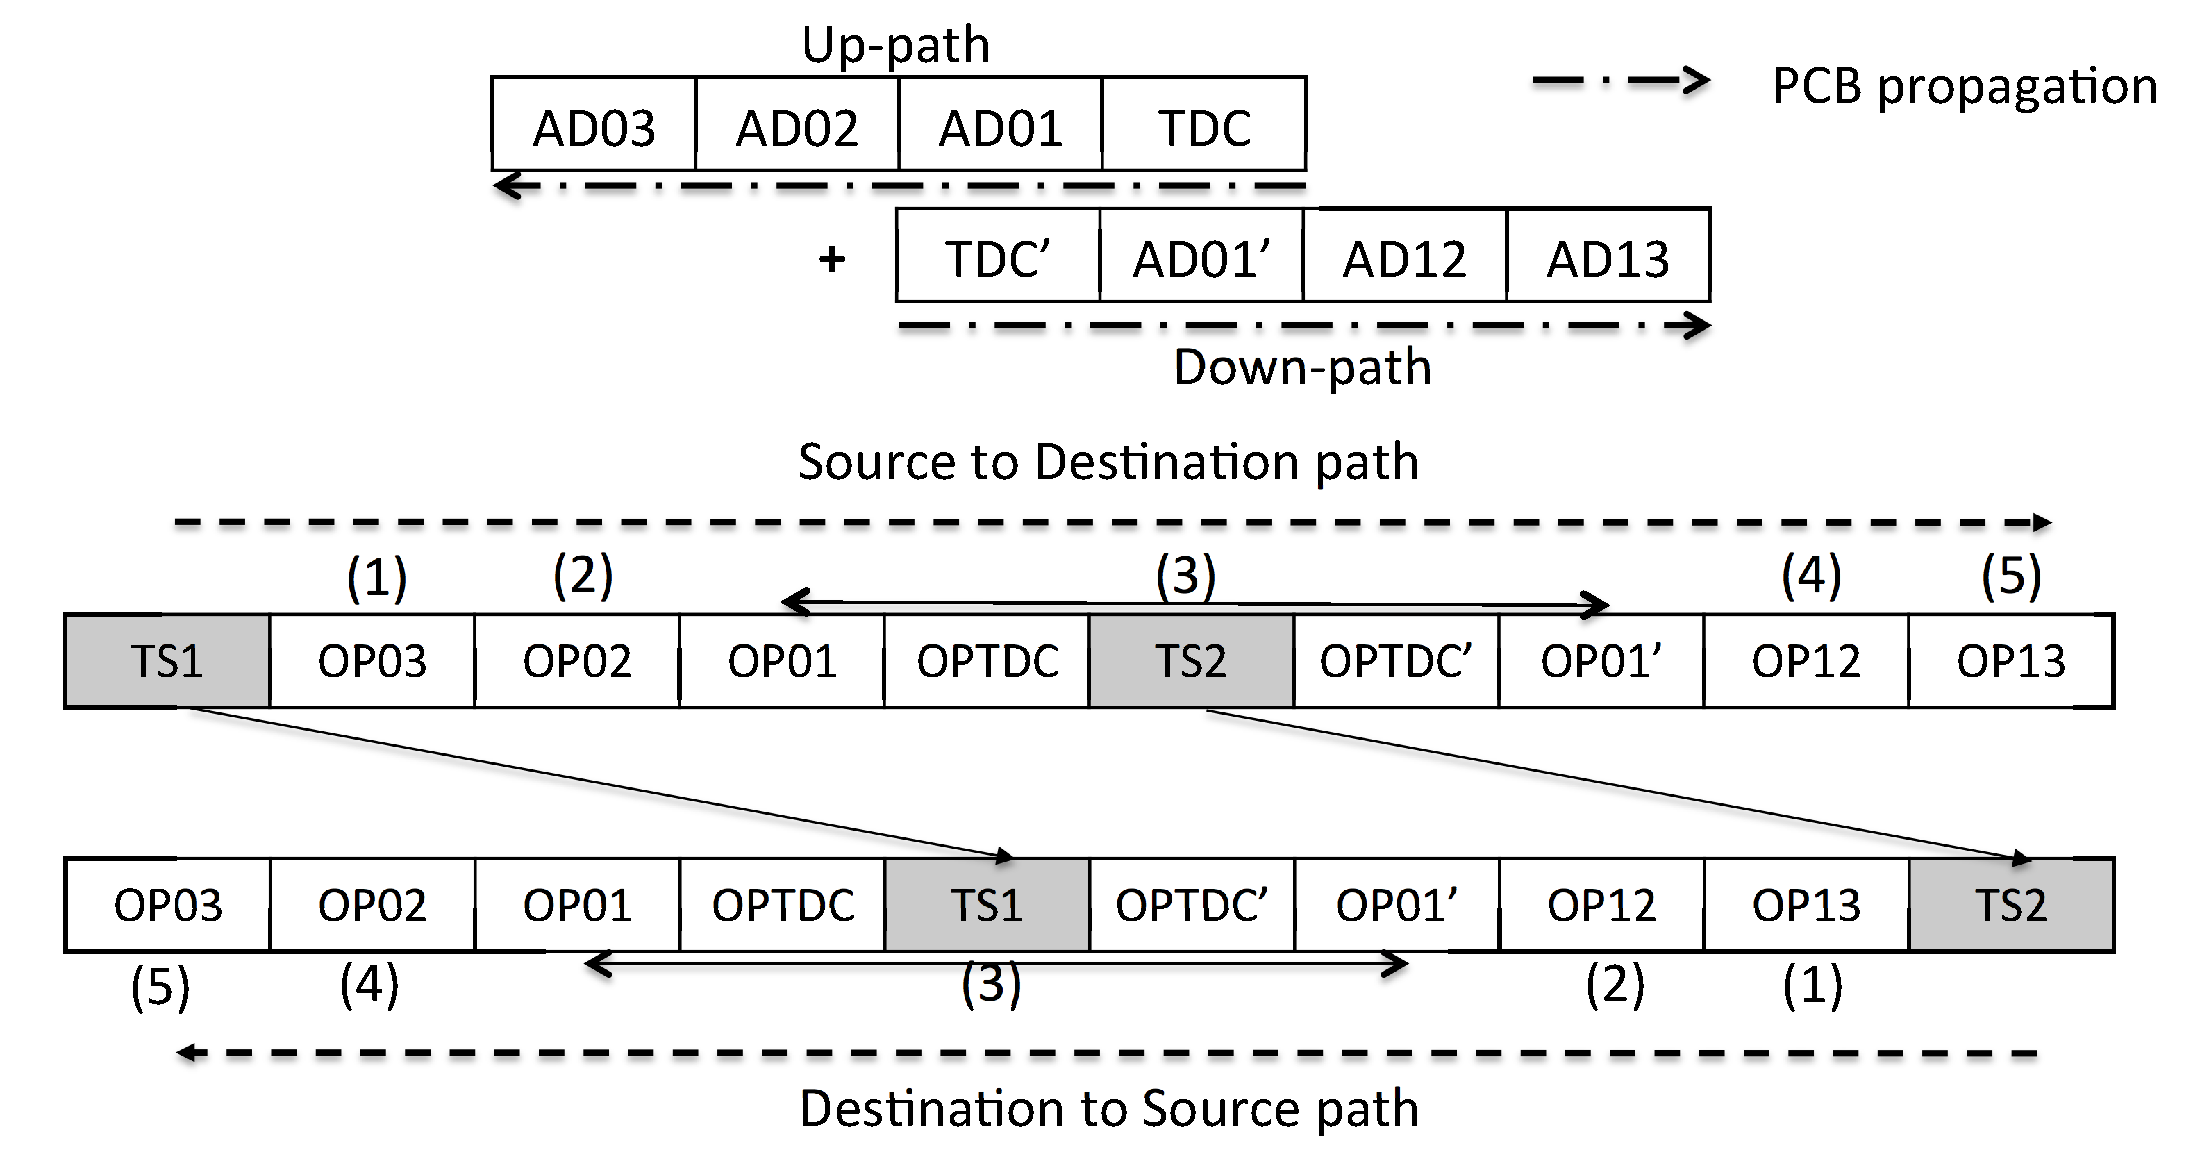
\includegraphics[width=.9\columnwidth]{./fig/nex_fwd2.eps}
\caption{Path composition through a rendezvous point.}\label{fig:ex-fwd-crossover}
\end{figure}

\noindent Figure~\ref{fig:ex-fwd-crossover} shows that \AD 01 is both on the up-path and down-path. In this case, a packet does not need to traverse \ISDC \AD, yet can be directly forwarded to to \AD 12 by \AD 01. To establish a shorter path, the sender sets the first 3 bits of the opaque field of \AD 01 to 110 (viz., Section~\ref{subsec:data-header}), to indicate that the \AD 01 is the common \AD of the up- and down-path (i.e., at the crossover point). If an ingress router finds it is on the crossover point, the router verifies its own opaque field, updates TS* to that of the down-path (which comes after TDC OPTDC in the figure), locates the next opaque field (that belongs to the egress router) coming after next three opaque fields (i.e., its parent, the special opaque field, and another opaque field of its parent), and forwards the packet to the egress interface. The ingress router has to update the Curr OF* to that of the egress router. Also, by having the ingress router update the TS*, the egress router processes this packet. The sender has to embed \ISDC's opaque fields (i.e., OPTDC and OPTDC') into the packet header so that the crossover \AD can verify the opaque fields generated by itself. We note that an \AD generates an opaque field using the opaque field marked by its provider as an input (i.e., by opaque field chaining), hence the provider's opaque field is necessary for opaque field verification.  


%3) Destination \AD is on the up-path.
\subsection{Destination \AD is on the up-path}

\begin{figure}[h]
\centering
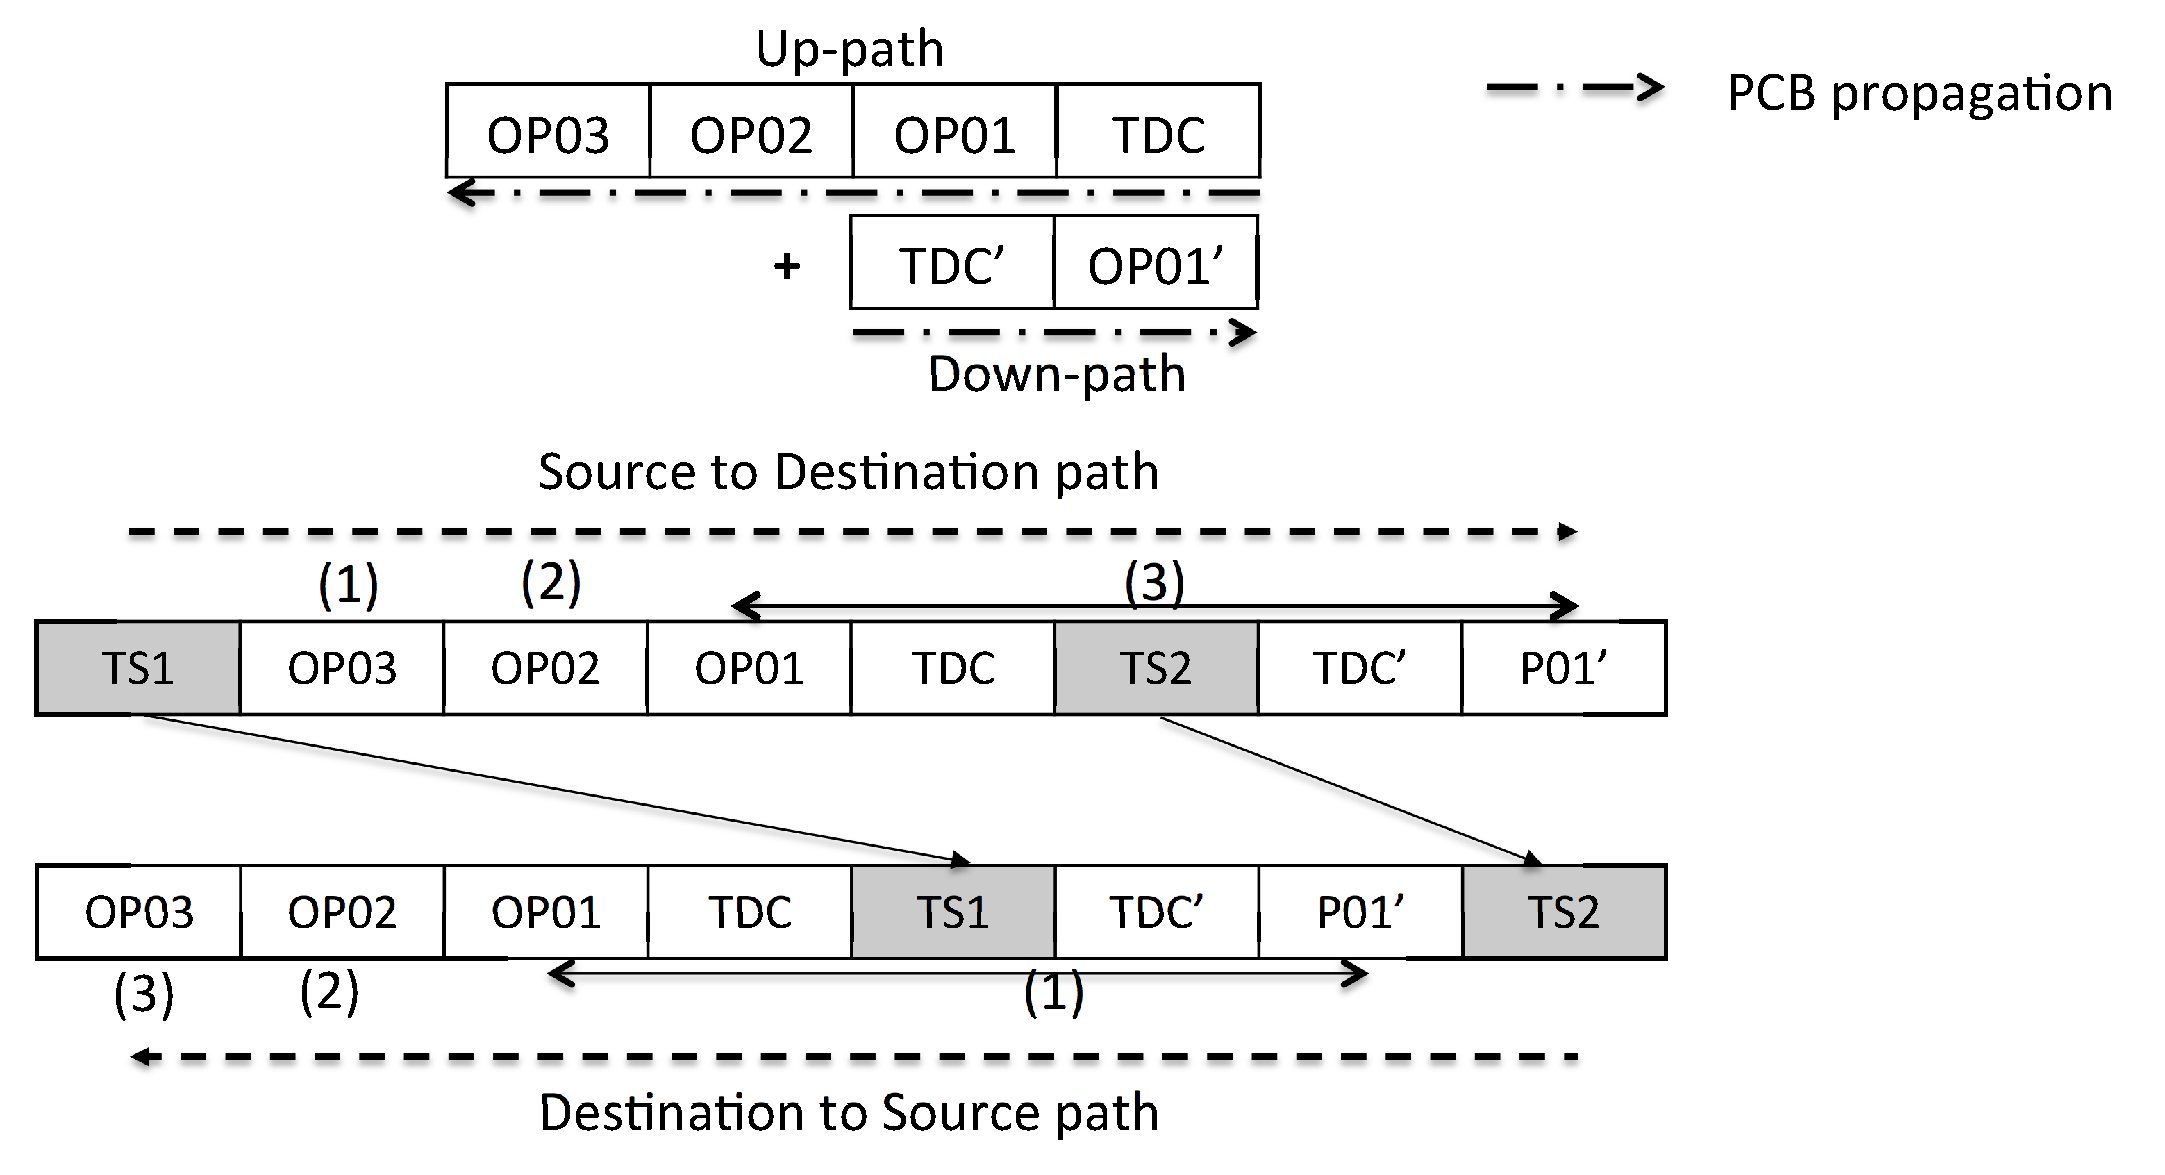
\includegraphics[width=.9\columnwidth]{./fig/nex_fwd3.eps}
\caption{Path composition on the same down-path.}\label{fig:ex-fwd-onpath}
\end{figure}

\noindent If the destination \AD is on the up-path, the sender composes the opaque field in the same way as the crossover scenario, yet the destination \AD is same as the crossover \AD. The destination \AD's down-path opaque field (i.e., OP01' in the figure) still needs to be present in the header so that \AD 01 verifies whether the path is constructed with a valid down-path.

%4) Up-path has a {\em shortcut} to an \AD in down-path.
\subsection{Up-path has a {\em shortcut} to an \AD in down-path}

\begin{figure}[h]
\centering
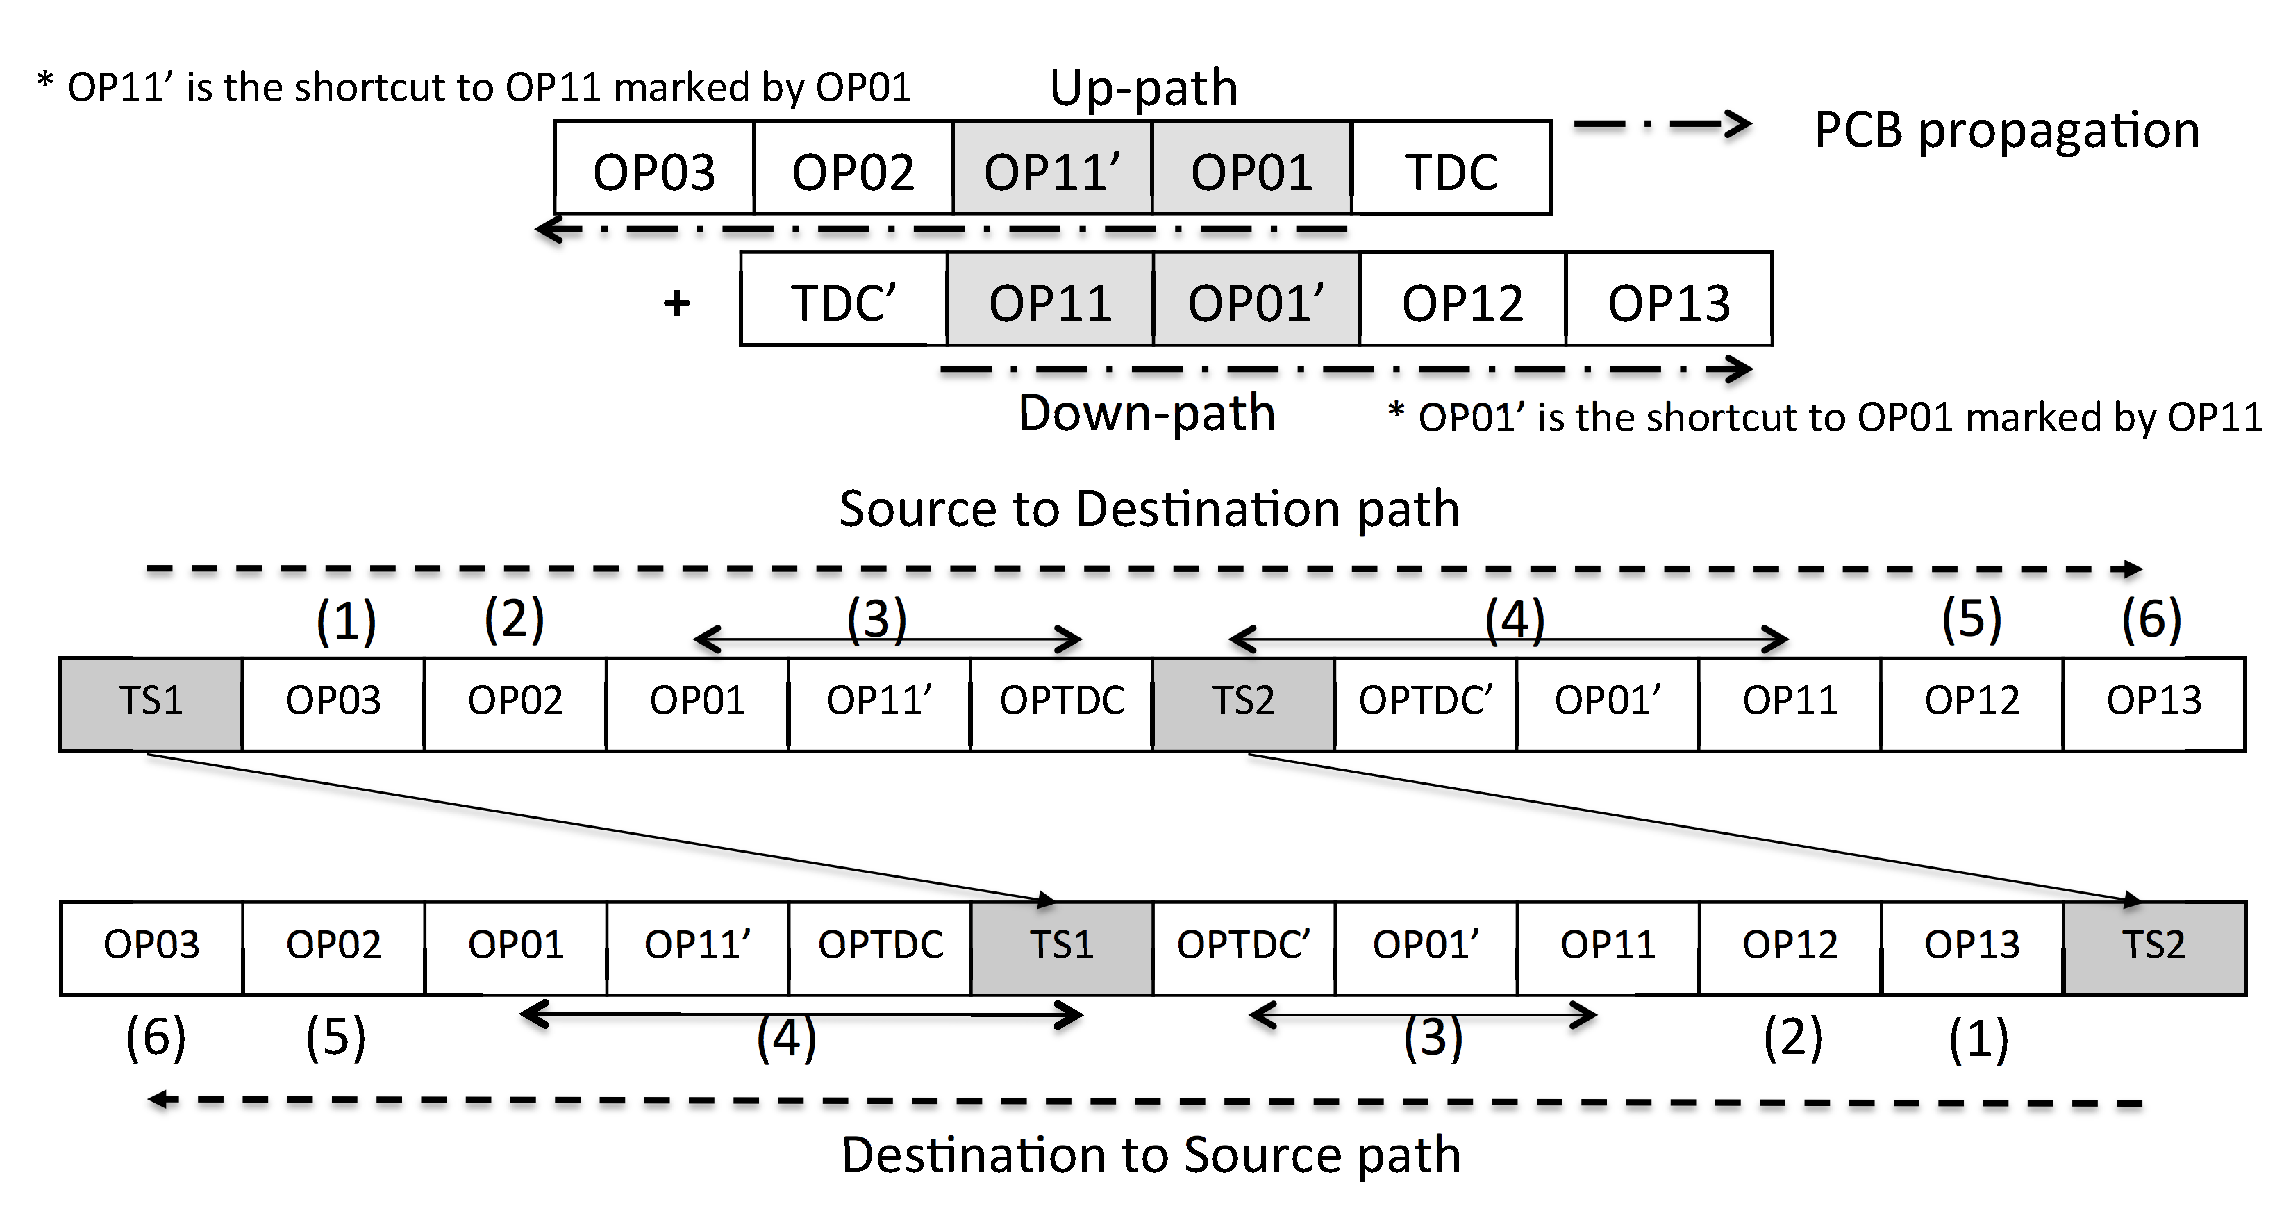
\includegraphics[width=.9\columnwidth]{./fig/nex_fwd4.eps}
\caption{Path composition through a shortcut.}\label{fig:ex-fwd-shortcut}
\end{figure}

\noindent Figure~\ref{fig:ex-fwd-shortcut} shows that during PCB propagation, \AD 01 added OP11' (i.e., shortcut path to \AD 11) to a PCB; and \AD 11 added OP01' (i.e., shortcut path to \AD 01) to a PCB. The sender constructs a shortcut path using the shortcut information (i.e., OP11' in this example) in the up- and down-path. The sender specifies its intent to use the shortcut by setting the first 4 bits of the opaque field (of the shortcut \AD) to 1111. Similar to the previous shortcut scenarios, the sender needs to include OP01 (which is chained to OP11' generation)  and OP11 (which is chained to OP01' generation) in the packet header to enable the \ADs at the crossover point (i.e., AD 01 and AD 12) to verify their opaque fields. However, different from the previous shortcut scenarios, the ingress router of the crossover \AD (i.e., \AD 01) has to skip OP01 and process with OP11' since OP01 is added for AD 02 to verify OP02. The same thing applies to the down-path, yet the first router of the down-path has to update the Curr OF* to that of AD 12 (i.e., OP12) so that the next \AD process the opaque field in the exactly same way as before (i.e., normally).

\begin{comment}
5) Up-path has a {\em shortcut} to an \AD in down-path and different \ISD (i.e., inter-ISD shortcut).
\begin{figure}[h]
\centering
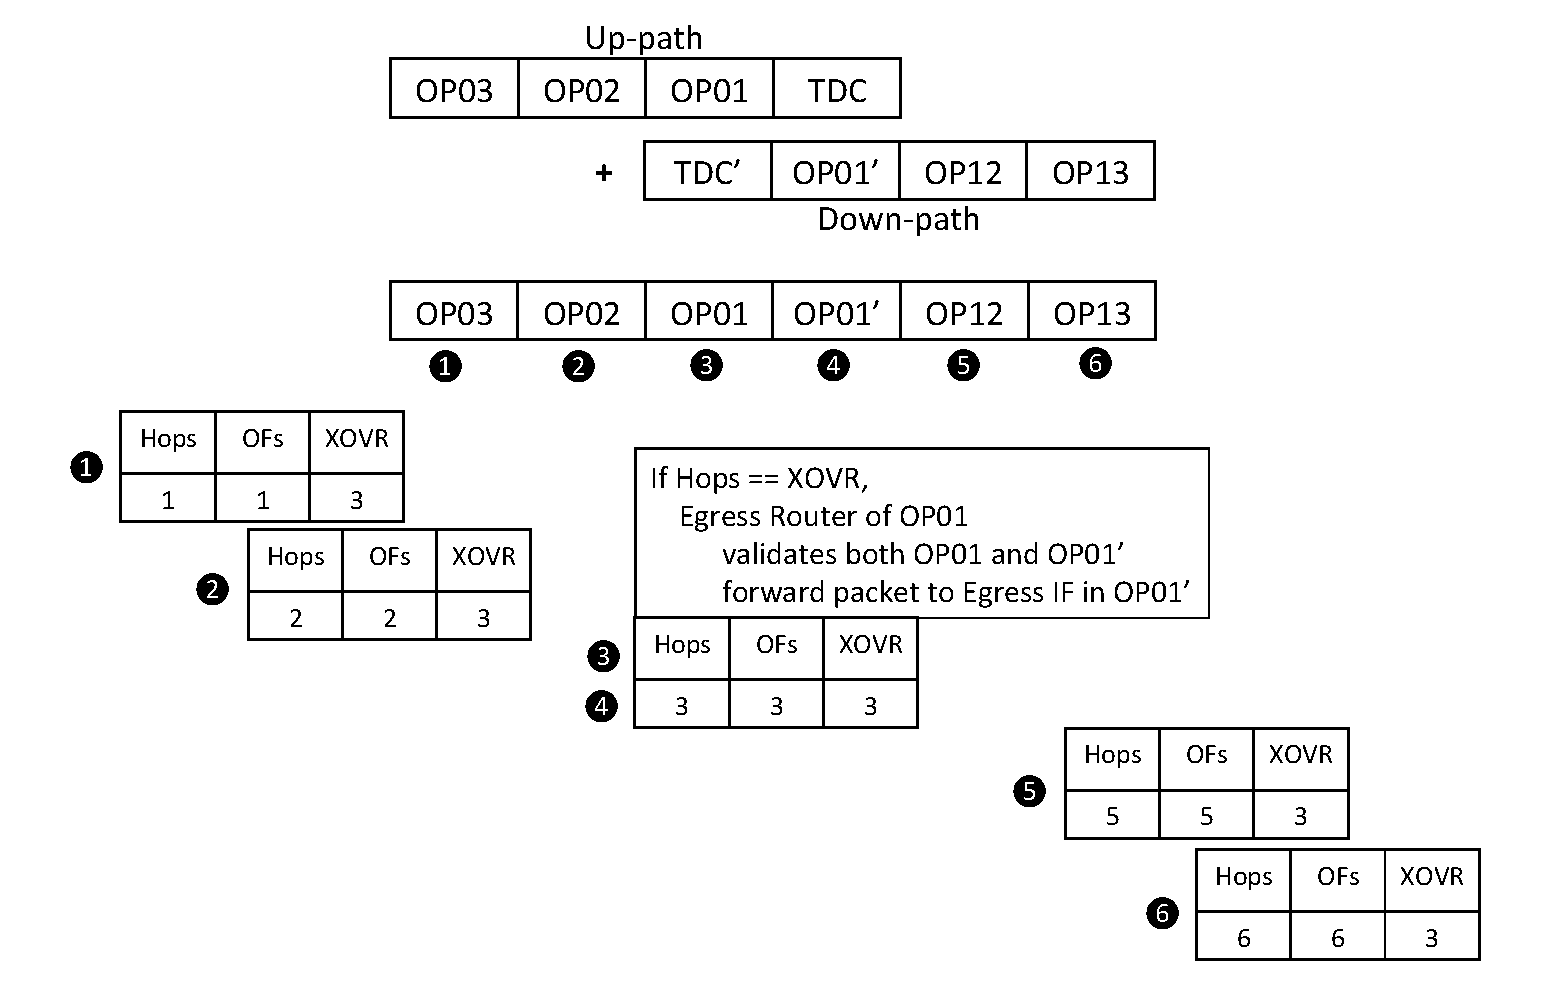
\includegraphics[width=.8\columnwidth]{./fig/ex_fwd5.eps}
\caption{Path composition through an inter-ISD shortcut.}\label{fig:ex-fwd-td-shortcut}
\end{figure}

Inter-ISD shortcut is 

\end{comment}
